\chapter{Margins}\label{ch:3}

As already mentioned, the main goal of this thesis is to provide empirical evidence regarding the quality of the simulation proposed in \cite{Urbano2018}. To this end, we can evaluate the statistical models that are used to perform the simulation, in terms of how well they fit (or describe) the data. We refer to this concept as \textit{goodness-of-fit}. If the models describe the data well, then consequently the simulation should be fairly realistic. 

As we discussed, the simulation relies on three models that are fitted separately: two margins and a copula. Conveniently, this also allows us to evaluate the margins separately from the copula. In this chapter, we explore how well the marginal distribution of system scores is modeled, independent of the copulas.

\section{Defining Goodness-of-Fit}

One simple approach for measuring the goodness-of-fit of a model would be to compute its Log-Likelihood (Equation \ref{eq:LL}). However this statistical measure is meaningful only for comparing two or more models. The absolute Log-Likelihood value in isolation is mostly meaningless. Furthermore, Log-Likelihood only measures how well the model fits the observed data; not how well it describes the underlying population. In other words, it does not measure the model's predictive power on unseen data.

Ideally, the best way to measure the goodness-of-fit of a fitted model $F^*$ is to compute its similarity to the \textit{true} distribution $F$ (the distribution of scores on the entire population of topics), also known as the \textit{ground truth}. Assuming that we have knowledge of the true distribution, there are several options for computing this similarity. We have considered three metrics that actually measure dissimilarity, which means that low values equate to high similarity. Namely, the \textit{i)} Kolmogorov–Smirnov (KS) statistic, \textit{ii)} Cramér–von Mises (CvM) criterion and \textit{iii)} Anderson–Darling (AD) statistic. All three of these metrics essentially define a distance $\Delta$ between the two cumulative distribution functions: $F^*$ and $F$.

The Kolmogorov–Smirnov (KS) statistic \cite{Kolmogorov1933, Smirnoff1939} is a simple metric which is defined as the largest absolute difference between two cumulative distribution functions across all $x$-values. The left plot of Figure \ref{fig:ks-and-cvm} shows the computed value of the KS statistic in one example. The value is the length of the red line.

\begin{equation}\label{eq:KS}
	\text{KS}\left(F^*, F\right) = \sup_x\left|F^*(x)-F(x)\right|
\end{equation}

The Cramér–von Mises (CvM) criterion \cite{VonMises1928} is defined as the squared area between the two curves. The right plot of Figure \ref{fig:ks-and-cvm} shows the computed value of the CvM statistic in one example. The value is the square of the red area.

\begin{equation}\label{eq:CvM}
	\text{CvM}\left(F^*, F\right) = \int_{-\infty}^{\infty}{\left[ F^*(x) - F(x) \right]^{2} dF^*(x)}
\end{equation}

Finally, the Anderson–Darling (AD) statistic \cite{Anderson1952} is defined similar to the CvM criterion. The main difference is that it places more weight on observations at the tails of the distribution, due to the $w(x)$ weighting function. When the weighting function is $w(x)=1$, the statistic is identical to the CvM criterion.

\begin{eqnarray}\label{eq:AD}
	\nonumber
	\text{AD}\left(F^*, F\right) = \int_{-\infty}^{\infty}{\left[ F^*(x) - F(x)\right]^{2}w(x)dF^*(x)},\\ 
	\textit{where } w(x)= \frac{1}{F^*(x)\left(1-F^*(x)\right)}	
\end{eqnarray}

\begin{figure}[t]
	\centering
	\begin{subfigure}{.4\textwidth}
		\centering
		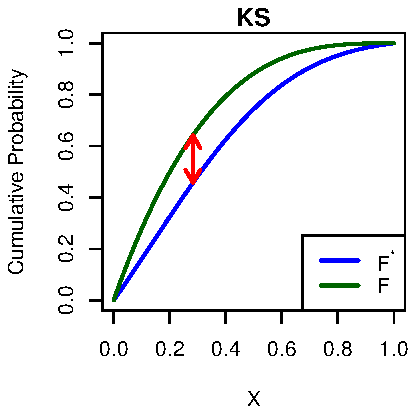
\includegraphics[width=0.95\linewidth]{margins/present_delta_KS_(m_cdf_A_T1_,m_cdf_A_T2)__ap}
	\end{subfigure}%
	\begin{subfigure}{.4\textwidth}
		\centering
		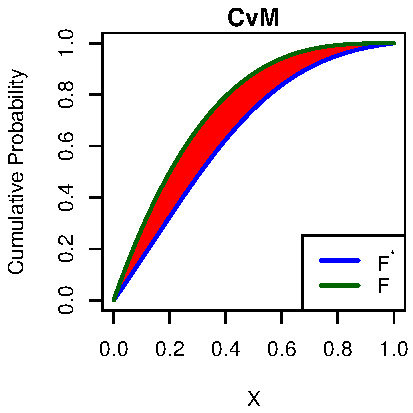
\includegraphics[width=0.95\linewidth]{margins/present_delta_cvm_(m_cdf_A_T1_,m_cdf_A_T2)__ap}
	\end{subfigure}
	\caption{Visualization of Kolmogorov–Smirnov statistic (left) and Cramér–von Mises criterion (right).}
	\label{fig:ks-and-cvm}
\end{figure}

In practice, having knowledge of the true distribution of a system's scores is not feasible, because it would imply that the system has been evaluated on the entire (possibly infinite) population of topics. This is either impractical due to the enormous amount of relevance judgments required, or even impossible if the potential set of topics is infinite or not well-defined. For this reason, some estimate of this true distribution is required.  

To this end, the so-called \textit{split-half} approach can be utilized, as schematically outlined in Figure \ref{fig:split-half-diag}. This approach is fairly common in the field of IR research \cite{Zobel1998, Voorhees2002, Urbano2013a, Sanderson2005, Cormack2007, Smucker2007}, and it is used in cases where obtaining ground truth data is too expensive or not feasible. Following this approach, the observations (in our case, the 50 topic-scores of a given system) are randomly split in two halves. The first half is treated as \textit{'the sample'} (the actual observations) and the second half as \textit{'the population'} (the ground truth). This means that for the purposes of measuring goodness-of-fit, the models are actually fitted on only the first half of the data. The empirical cumulative distribution ECDF of the second half of the data is used as an estimate of the true distribution (the ground truth). We use $F_1^*$ to denote the distribution of the fitted model and $F_2$ to denote the estimated true distribution. In order to measure the goodness-of-fit of the model $F_1^*$, we can use any of the three aforementioned metrics (Equations \ref{eq:KS}-\ref{eq:AD}). 

\begin{figure}[t]
	\centering	
	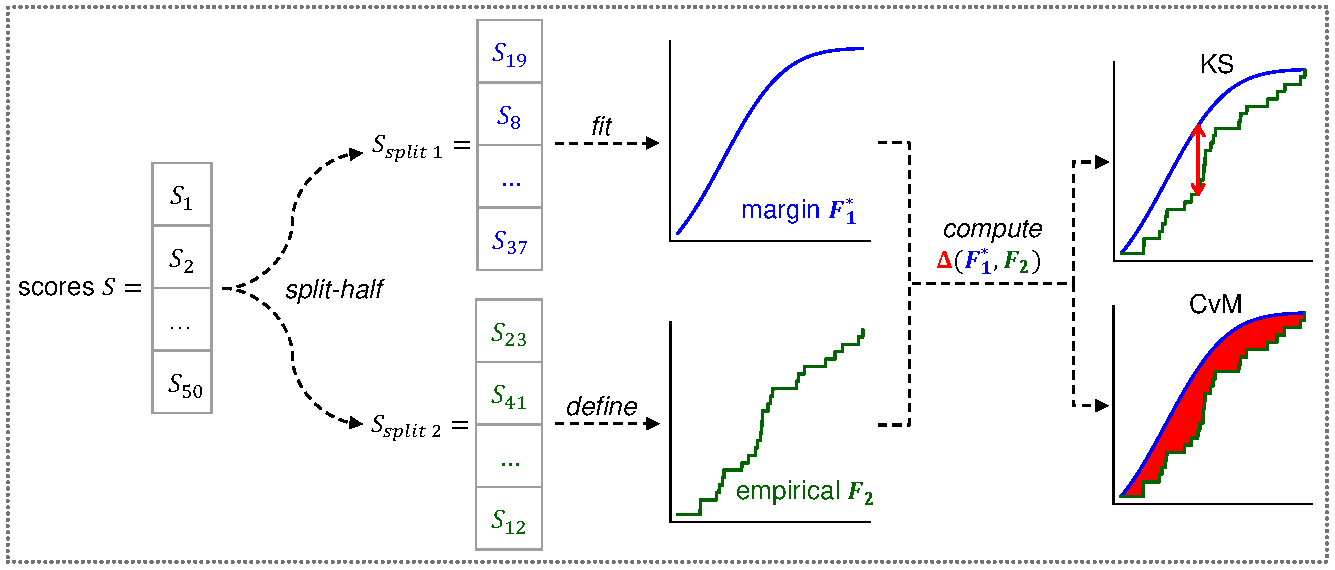
\includegraphics[width=1\linewidth]{../diagrams/diag2_splithalf}
	\caption{Diagrammatic representation of the Split-Half approach.}
	\label{fig:split-half-diag}
\end{figure}

For our purposes, there is likely no benefit in placing more weight on the tails of the distribution, or only considering the largest distance. Therefore, the CvM criterion (Equation \ref{eq:CvM}) can be safely chosen as the measure of choice. We use $\Delta_\text{obs}$ to denote the observed distance (or dissimilarity) between a fitted model and the estimated ground truth, that corresponds to a given random split. Intuitively, it represents the area between the two curves.

\begin{equation}\label{eq:Delta_obs}
	\Delta_\text{obs} = \sqrt{\text{CvM}\left(F_1^*, F_2\right)}
\end{equation}

%\begin{eqnarray}\label{eq:Delta_obs}
%	\Delta_\text{obs} = \sqrt{\text{CvM}\left(F_1^*, F_2\right)} = \sqrt{\int_{-\infty}^{\infty}{\left[ F_1^*(x) - F_2(x) \right]^{2} dF_1^*(x)}}
%\end{eqnarray}

Utilizing $\Delta_\text{obs}$, the goodness-of-fit of a model $F_1^*$ can simply be defined as its $-\Delta_\text{obs}$. The minus sign is due to the fact that the goodness-of-fit of a model and its deviation from the ground truth are inversely related. 

As an example, in Figure \ref{fig:motivate_delta_exp_A} we show the computed $\Delta_\text{obs}$ values of two models in one particular split. One limitation regarding the interpretation of these measurements, is that it is not obvious which specific range of values constitute a good fit. In relative terms, we could say that the model with the lowest $\Delta_\text{obs}$, in this case 0.05, is better. However, in absolute terms, it is not obvious how to assess if the model that measured $\Delta_\text{obs}=0.05$ constitutes a good fit or not. To overcome this problem, we need to determine what value we should approximately expect from a good fit. We use $\Delta_\text{exp}$ to denote this value.

\begin{figure}[t]	
	\centering
	\begin{subfigure}{.666\textwidth}
		\begin{subfigure}{.5\textwidth}
			\centering
			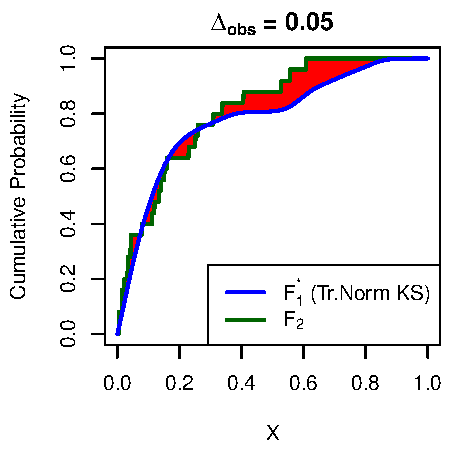
\includegraphics[width=0.95\linewidth]{margins/need_for_Dexp_(ap)1}
		\end{subfigure}%
		\begin{subfigure}{.5\textwidth}
			\centering
			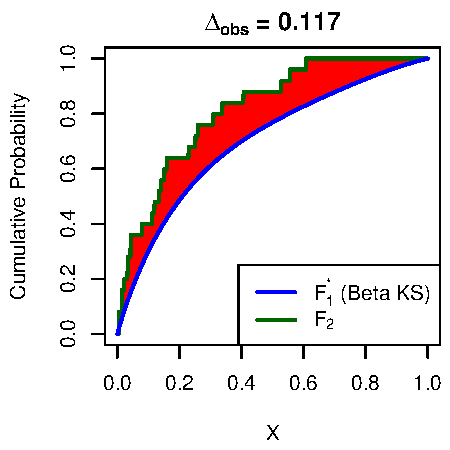
\includegraphics[width=0.95\linewidth]{margins/need_for_Dexp_(ap)2}
		\end{subfigure}%	
		\caption{}
		\label{fig:motivate_delta_exp_A}
	\end{subfigure}%
	\begin{subfigure}{.333\textwidth}
		\centering
		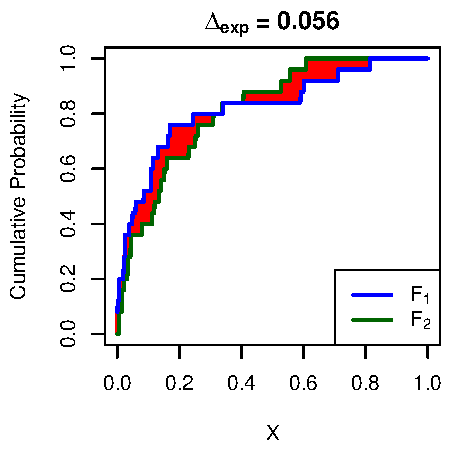
\includegraphics[width=0.95\linewidth]{margins/need_for_Dexp_(ap)3}		
		\caption{}
		\label{fig:motivate_delta_exp_B}
	\end{subfigure}
	\caption{Visualization of: (\subref{fig:motivate_delta_exp_A}) the $\Delta_\text{obs}$ of two models on the same split, and (\subref{fig:motivate_delta_exp_B}) corresponding $\Delta_\text{exp}$.}
\end{figure}

One way of calculating this $\Delta_\text{exp}$, is to measure the distance that would have been observed if the empirical distribution of the first half of the data ($F_1$) was used instead of the fitted model, as shown in Figure \ref{fig:gof_diagram}. 

\begin{equation}\label{eq:Delta_exp}
	\Delta_\text{exp} = \sqrt{\text{CvM}\left(F_1, F_2\right)}
\end{equation}

The advantage of using the empirical distribution as a \textit{reference}, is that it gives us an unbiased measurement, because it is not based on any model. Using this definition, in this particular example, $\Delta_\text{exp}$ was measured to be $0.56$ (Figure \ref{fig:motivate_delta_exp_B}), which is actually higher than $0.05$. This implies that the fit was slightly better than our expectation. In general, a model that fits the data well should measure a $\Delta_\text{obs}$ that is about the same as its corresponding expectation $\Delta_\text{exp}$. 

\begin{figure}[t]
	\centering	
	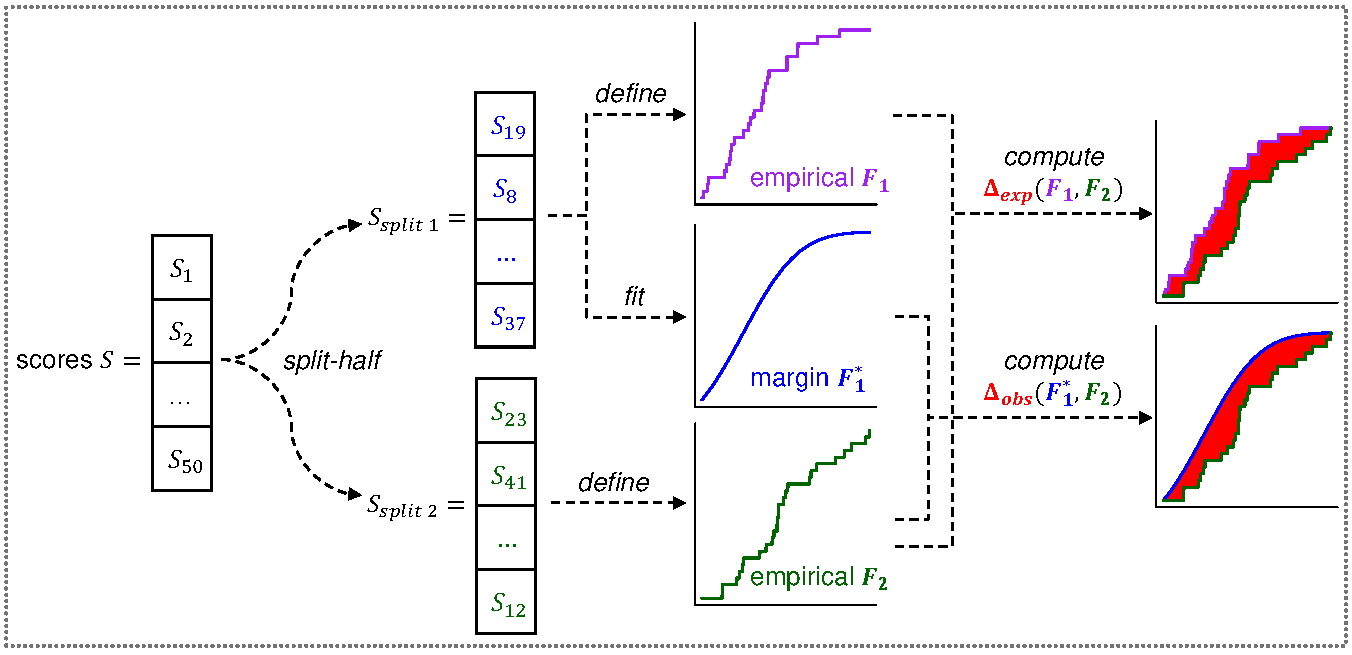
\includegraphics[width=1.0\linewidth]{../diagrams/diag3_gof}
	\caption{Diagrammatic representation of $\Delta_\text{obs}$ and $\Delta_\text{exp}$.}
	\label{fig:gof_diagram}
\end{figure}

\section{Experiments}

For our experiments, we require existing collections of evaluation scores of systems on topics, so that models can be fitted on real data. The collections we use throughout this thesis come from actual results of systems that TREC participants submitted in previous years, in the Ad-hoc and Web track, as detailed in Table \ref{tab:dataset-descriptive-stats}. This dataset contains a large number of systems, as well as a wide range of effectiveness measures, namely: AP, nDCG@20, ERR@20, P@10 and RR. This ensures that the quality of the stochastic simulation is explored on a variety of IR data. We pre-process the data by removing the bottom 10\% performing systems, to avoid erroneous system implementations, so the final number of systems is slightly smaller.

\begin{table}[t]
	\centering
	\begin{tabular}{l c c c l}
		\toprule
		TREC Track & Years & \#Systems & \#Topics & Effectiveness Measures \\
		\midrule
		Ad-hoc & 2005 to 2008 & 363 & 50 & \{AP, RR, P@10\} \\
		Web & 2010 to 2013 & 216 & 50 & \{nDCG@20, ERR@20\} \\
		%		Terabyte & 2006 & 61 & 149 & \{AP, RR, P@10\} \\
		\bottomrule
	\end{tabular}
	\caption{Some descriptive statistics about the data collections.}
	\label{tab:dataset-descriptive-stats}
\end{table} 

Our primary objective is to measure how well can we capture the marginal distribution of scores, of a given system. To this end, for each effectiveness measure, we select a random system from a random collection and perform the aforementioned split-half approach using the system's scores on all (50) topics. In total, \num{250000} splits were performed; \num{50000} for each effectiveness measure. This amount of splits seems to be sufficient, judging from the narrow confidence intervals we obtain for most of our results. For each split, we calculate a corresponding $\Delta_{\text{exp}}$ (Equation \ref{eq:Delta_exp}). Then, using the data in the first half of the split, we fit all possible models according to Table \ref{tab:fams} and compute their corresponding $\Delta_{\text{obs}}$ (Equation \ref{eq:Delta_obs}). 

Figure \ref{fig:example-m-delta-computations} shows the $\Delta_{\text{obs}}$ (left) and $\Delta_{\text{exp}}$ (right) for two example random splits. The approach used for computing these values is slightly different depending on whether the data are continuous (AP, nDCG@20, ERR@20) or discrete (P@10, RR). For the case of continuous measures, we use an estimation approach by averaging the absolute differences between the two curves across 1000 equally spaced $x$-values in the $\left[0,1\right]$ range. For the case of discrete measures, we average the absolute differences between the two curves across all possible $x$-values. P@10 has 11 possible values: ${\{0, 0.1, 0.2, \dots, 1\}}$, whereas RR has 1001. In the first example (Figure \ref{fig:example-m-computations-ap}), the effectiveness measure was AP (continuous metric) and the Truncated Normal Kernel Smoothing distribution was selected. The model performed worse than the expectation (0.064 > 0.048). In the second example (Figure \ref{fig:example-m-computations-p10}), the effectiveness measure was P@10 (discrete metric) and the Beta-Binomial distribution was selected. The model performed better than our expectation (0.04 < 0.047). 

\begin{figure}[t]
	\centering
	\begin{subfigure}{\textwidth}
		\centering
		\begin{subfigure}{.4\textwidth}
			\centering
			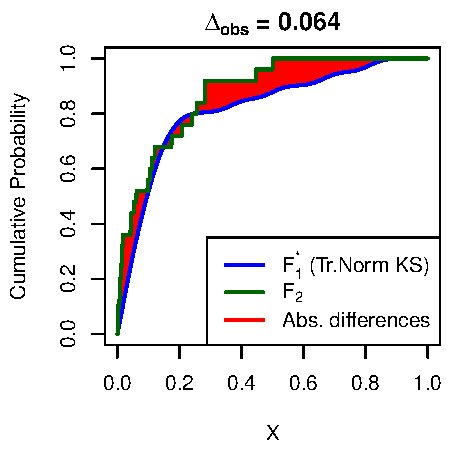
\includegraphics[width=0.90\linewidth]{margins/example_Dobs_ap}
		\end{subfigure}%
		\begin{subfigure}{.4\textwidth}
			\centering
			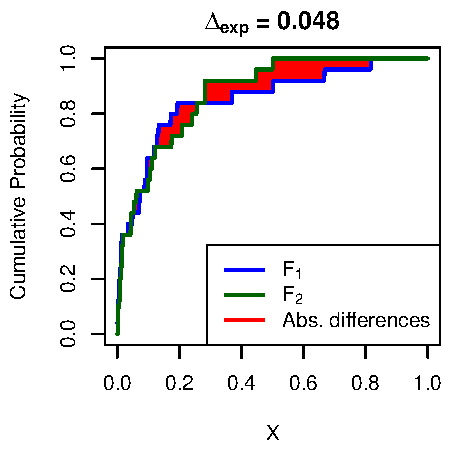
\includegraphics[width=0.90\linewidth]{margins/example_Dexp_ap}
		\end{subfigure}
		\caption{Example random split using the AP scores of system 91 on the 50 topics of the Ad-hoc 2008 test collection.}
		\label{fig:example-m-computations-ap}
	\end{subfigure}
	
	\begin{subfigure}{\textwidth}
		\centering
		\begin{subfigure}{.4\textwidth}
			\centering
			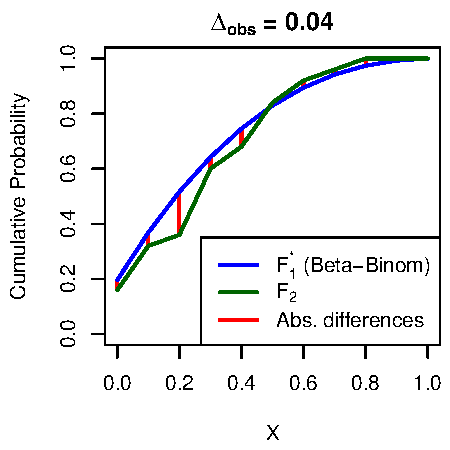
\includegraphics[width=0.90\linewidth]{margins/example_Dobs_p10}
		\end{subfigure}%
		\begin{subfigure}{.4\textwidth}
			\centering
			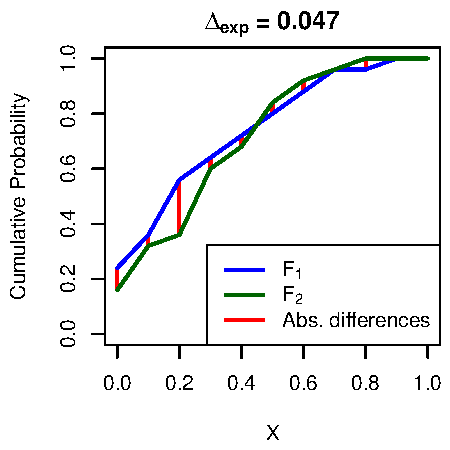
\includegraphics[width=0.90\linewidth]{margins/example_Dexp_p10}
		\end{subfigure}
		\caption{Example random split using the P@10 scores of system 107 on the 50 topics of the Ad-hoc 2008 test collection.}
		\label{fig:example-m-computations-p10}
	\end{subfigure}	
	
	\caption{Visualization of $\Delta_{\text{obs}}$ (left) and $\Delta_{\text{exp}}$ (right) for: (\subref{fig:example-m-computations-ap}) the continuous case using AP scores, and (\subref{fig:example-m-computations-p10}) the discrete case using P@10 scores.}
	\label{fig:example-m-delta-computations}
\end{figure}

In Figure \ref{fig:margins-splithalf-plot-1&2} we report the results across all \num{250000} random splits, separately for each effectiveness measure and family of distribution. All model selections were made according to AIC, as done in \cite{Urbano2019}. The left plot shows the mean values of $\Delta_{\text{obs}}$ and $\Delta_{\text{exp}}$. In general, models that fit the data well should give us $\Delta_{\text{obs}}$ values about the same as their corresponding expected value $\Delta_{\text{exp}}$. In order to make it easier to visually interpret the results, we have defined a goodness-of-fit metric, denoted as \textit{GoF}, that combines $\Delta_{\text{obs}}$ and $\Delta_{\text{exp}}$ in a single formula, as the (negative\footnote{This is because the goodness-of-fit of a model and its deviation from the ground truth are inversely related.} of the) percentage deviation of $\Delta_\text{obs}$ from the corresponding expected value $\Delta_\text{exp}$:

\begin{eqnarray}\label{eq:gof}
	\text{GoF} = -\frac{\Delta_\text{obs} - \Delta_\text{exp}}{\Delta_\text{exp}}    	
\end{eqnarray}

The interpretation of GoF is quite straightforward. For example, when GoF is -0.333 (Figure \ref{fig:example-m-computations-ap}), this means that $\Delta_\text{obs}$ is 33.3\% higher than the expectation. Similarly, when GoF is 0.149 (Figure \ref{fig:example-m-computations-p10}), this means that $\Delta_\text{obs}$ is 14.9\% lower than the expectation.

\begin{figure}[t]
	\centering	
	\begin{subfigure}[t]{.45\textwidth}
		\centering
		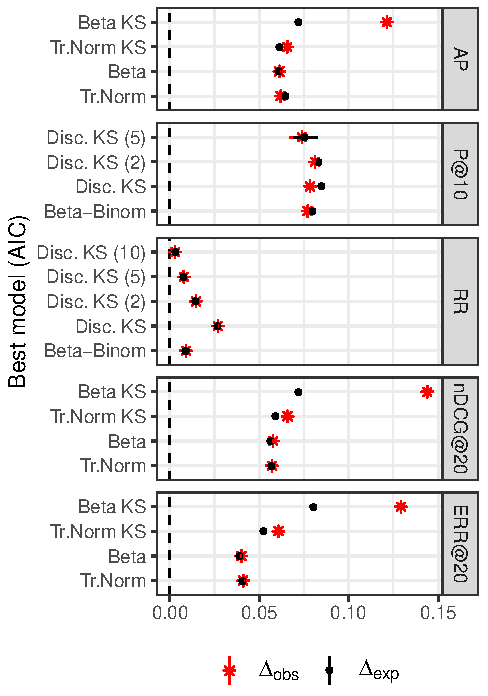
\includegraphics[scale=0.85,valign=t]{margins/splithalf_n250000_fig1}
		%		\caption{}
		%		\label{fig:margins-splithalf-plot-1}
	\end{subfigure}%
	\begin{subfigure}[t]{.45\textwidth}
		\centering
		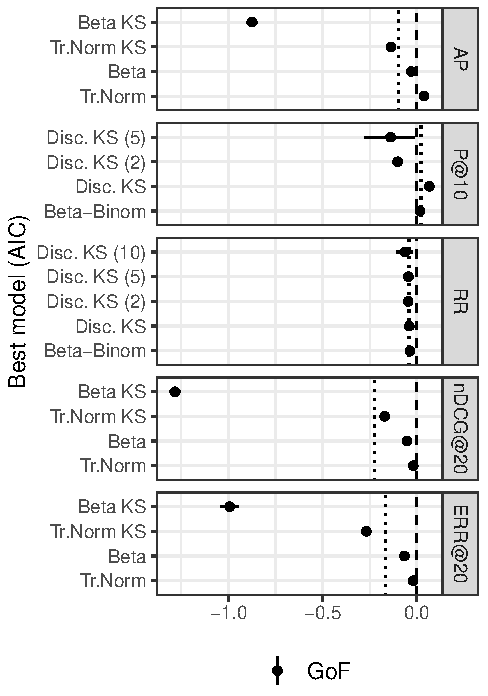
\includegraphics[scale=0.85,valign=t]{margins/splithalf_n250000_fig2}
		%		\caption{}
		%		\label{fig:margins-splithalf-plot-2}
	\end{subfigure}
	\caption{How well does each family of marginal distributions perform, when it is selected by AIC? Mean values are reported, along with 95\% bootstrap confidence intervals. The dotted vertical lines (on the right plot) indicate the overall means across each effectiveness measure.}
	\label{fig:margins-splithalf-plot-1&2}
\end{figure}

\begin{figure}[!t]
	\centering	
	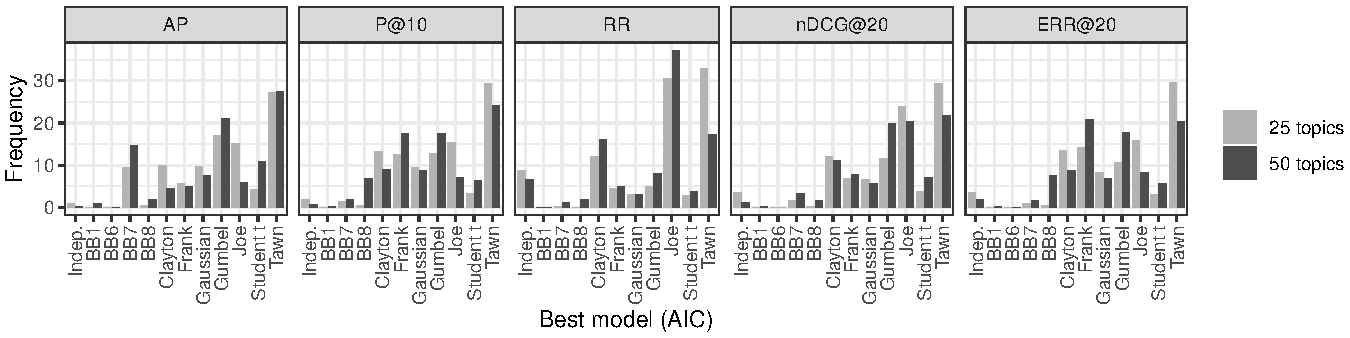
\includegraphics[scale=0.8]{margins/splithalf_n250000_fig3}
	\caption{Frequency with which each candidate family of marginal distributions is selected by AIC. We consider the case where models are fitted on 25 and 50 topics respectively.}
	\label{fig:margins-splithalf-plot-3}
\end{figure}

Overall, our results show that the average GoF is slightly less than zero across the board, with the exception of the Beta Kernel Smoothing distribution family. Ideally, we want to observe values close to zero. These results suggest that the models provide a moderately good fit, however there is certainly room for improvement. Moreover, we notice that the models fit discrete metrics (P@10 and RR) noticeably better than continuous (AP, nDCG@20 and ERR@20).

Figure \ref{fig:margins-splithalf-plot-3} shows the frequency with which each candidate family is selected. One side-effect of employing a split-half approach is that the data are being halved, which means that our marginal models are actually fitted on only 25 topic-scores, instead of the entire set of 50 topic-scores. However, we are truly interested in measuring the goodness-of-fit of models that are fitted on 50 scores, as opposed to 25. For this reason, our plot shows the frequency with which each candidate family is selected, when the models are fitted on \textit{i)} 25, as well as \textit{ii)} 50 scores. It appears that the models are selected very similarly in both cases, except for two Discrete Kernel Smoothing variants in the case of P@10. This increases our level of confidence regarding the accuracy of our estimates of goodness-of-fit. Furthermore, since all candidate families get selected, and no particular family gets chosen with a significantly higher frequency than the rest; this reaffirms the idea that IR data are quite complex, as it implies that a variety of marginal models is required, to describe IR data. 

The Beta KS distribution family is an obvious outlier with an average GoF of about -1; which means that the average $\Delta_{\text{obs}}$ is twice what we expected. This would not be a problem, if that average $\Delta_{\text{obs}}$ was a very low value, but as we can see in the left plot this is not the case. It is actually the highest across all (continuous) effectiveness measures. There are two possible explanations for this. One possible explanation is that our model selection criterion (AIC) made a poor choice by choosing this particular distribution family, which means that some other candidate family would have performed better if it had been properly selected. Another possible explanation is that this particular set of random splits is a corner case where none of the candidate families that are incorporated in the simulation would have performed well, and Beta KS just happened to be the lesser bad choice. As we can see in Table \ref{tab:bks-freq}, Beta KS is not selected very frequently. Overall, it is selected 9.59\% of the times where it is eligible for selection. Even though this not a particularly high percentage, dealing with this outlier could considerably improve the quality of the simulation. It is therefore meaningful to explore this further.



\begin{table}[t]
	\centering
	\begin{tabular}{c c c} % middle column is all italic
		\toprule
		& \textit{25 topics} & \textit{50 topics} \\
		\midrule
		AP          & 6.43\%  & 8.58\% \\ 
		nDCG@20     & 11.9\%  & 18.6\% \\
		ERR@20      & 3.96\%  & 1.56\% \\
		\midrule
		Overall     & 7.44\% & 9.59\% \\
		\bottomrule
	\end{tabular}
	\caption{How often is Beta KS selected by AIC? We consider the case where models are fitted on 25 and 50 topics respectively.}
	\label{tab:bks-freq}
\end{table}

In an effort to explain why the Beta KS distribution performs poorly on average, even though AIC ranks it \nth{1}, we experimented by comparing a few cases where it performed well, with cases where it performed poorly, at the extremes. Figure \ref{fig:bks-good-vs-bad} illustrates two of those example cases, where Beta KS provided a good fit (left) and a bad fit (right), respectively. These examples were hand-selected to demonstrate a noticeable pattern that we observed through our exploratory experimentation. In both examples, we see that Beta KS has trouble fitting the data, when the number of zero values (in this case, nDCG@20 scores) is too large. This is because the fitted models tend to be too simple, as evident by the low \textit{effective degrees of freedom} (edf) of \num{2.5} and \num{2.4} respectively. In other words, Beta KS is not a complex enough model to capture the high appearance of zeros in the data. Despite this, in both examples, AIC selected these simple yet seriously underfitted Beta KS models. Looking at the right-hand side plot, we see that Beta KS does not describe the ground truth data well, measuring $\Delta_{\text{obs}}=0.16$. In contrast, Log-Likelihood would have made a better choice, namely Truncated Normal KS, that would have measured $\Delta_{\text{obs}}=0.07$. However, since none of the model selection criteria are perfect, this is not entirely surprising. Looking at the left-hand side plot, we see that the reason why Beta KS sometimes performs well, in this case measuring $\Delta_{\text{obs}}=0.04$, is simply due to chance. More specifically, due to the randomness of splitting the data in half, sometimes one of the data halves contains many more zero values than the other half. If the zeros are present mostly in the first half, the underfitted Beta KS model describes the ground truth data well, due to chance. In summary, we found that in certain corner cases (i.e., when the appearance of zeros in the data is high), AIC tends to select Beta KS due to its low complexity, despite the model being underfitted, which often results in high $\Delta_{\text{obs}}$ measurements.

\begin{figure}[t]
	\centering
	\begin{subfigure}{.48\textwidth}
		\centering	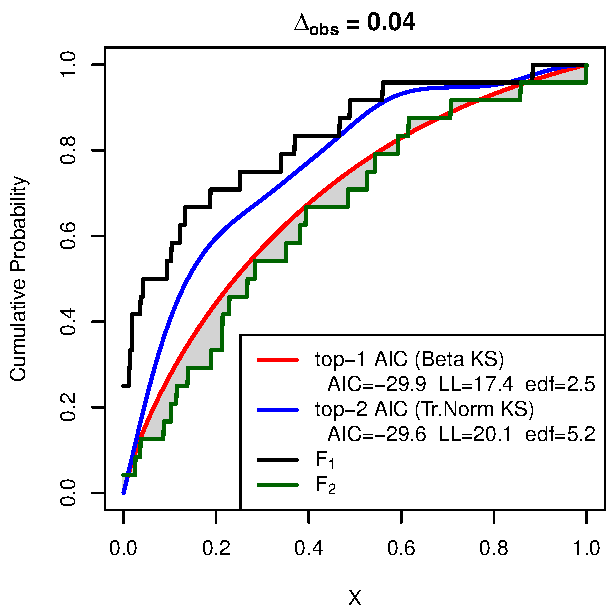
\includegraphics[width=0.95\linewidth]{margins/explore_bks_performance/best_9833_ndcg20}
	\end{subfigure}%
	\begin{subfigure}{.48\textwidth}
		\centering
		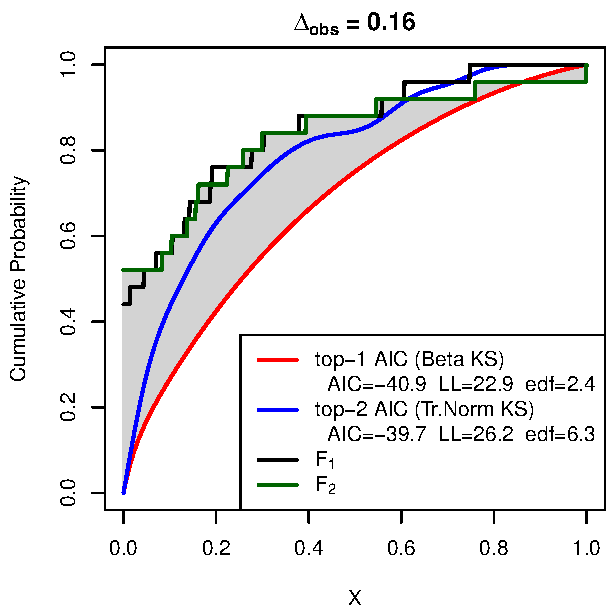
\includegraphics[width=0.95\linewidth]{margins/explore_bks_performance/worst12_ndcg20}
	\end{subfigure}
	\caption{Visualization of two example Beta KS fits: a good fit (left), and a bad fit (right).}
	\label{fig:bks-good-vs-bad}
\end{figure}

Based on our exploratory experimentation, we speculated that the large number of zero scores in the data causes outliers in our results. To further verify this, in Figure \ref{fig:margins-splithalf-plot-7} we compare those specific random splits where AIC selected Beta KS (we refer to those cases as 'corner cases'), with all other cases. In the top plot, we see that for the case of nDCG@20 (which is actually the most common case, as per Table \ref{tab:bks-freq}), the number of zeros in the data is significantly larger in these corner cases, compared to all other cases. This is in line with our previous findings. However, this is not true for AP and ERR@20, which means that there are other particularities about these corner cases, beyond the high appearance of zeros, which we did not manage to identify through our exploratory experimentation. In the middle and bottom plots, we show the theoretical minimum $\Delta_{\text{obs}}$ and maximum GoF, that would have been achieved if the candidate models had been selected in an optimal manner. This was done by simply selecting the model with the lowest $\Delta_{\text{obs}}$ in each random split. It appears that even the best possible candidate would not have performed well in the corner cases; in both absolute terms ($\Delta_{\text{obs}}$), and terms relative to the expectation (GoF). This suggests that additional candidate models would have been required, to achieve a good fit. One possible addition of such candidate could be a mixture model, that models the zero scores separately from non-zeros. However, we leave this for future work. 

\begin{figure}[t]
	\centering	
	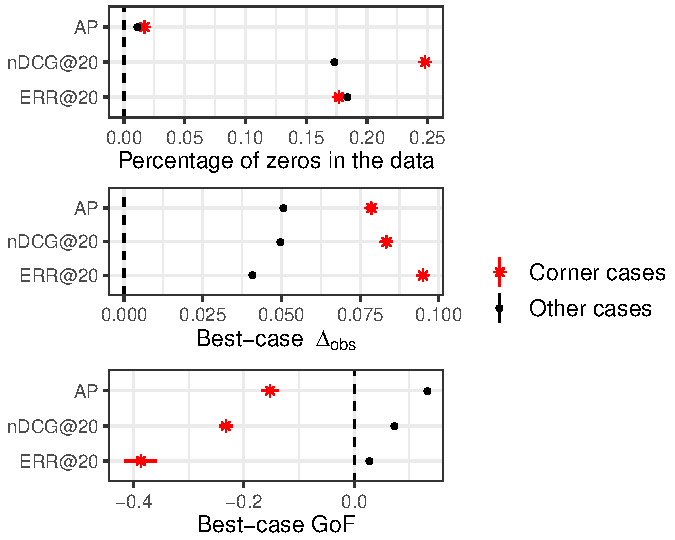
\includegraphics[scale=0.9]{margins/splithalf_n250000_fig7}
	\caption{Comparing the cases where AIC ranked Beta KS \nth{1}, with all other cases.}
	\label{fig:margins-splithalf-plot-7}
\end{figure}

In Figure \ref{fig:splithalf_n250000_figa1}, we see a clear correlation between the appearance of zeros in the data, and goodness-of-fit; both in absolute terms ($\Delta_{\text{obs}}$), and terms relative to the expectation (GoF). This further verifies our hypothesis that data containing a high number of zeros are not modeled properly.
	

In an attempt to correct the outliers in our results, we continue to focus on these corner cases where AIC determined that Beta KS was the best candidate model. One possible starting point (that does not involve expanding the list of candidate models) is to investigate if the removal of the Beta KS distribution from the list of candidates, would have resulted in an overall improvement, in terms of overall mean $\Delta_{\text{obs}}$. This is the equivalent of selecting the \nth{2} best model according to AIC, since we are now only focusing on the specific splits where Beta KS was ranked \nth{1}. We also include the \nth{3} best model in the comparison, to verify if it is indeed worse than the \nth{2} best. Figure \ref{fig:margins-splithalf-plot-4} verifies that the \nth{2} best model is indeed better than the \nth{3} best, by a significant margin. However, Beta KS does not provide a good fit on average. In fact, surprisingly, both the \nth{2} best and \nth{3} best models provide a better fit, with only one exception in the case of ERR@20. Moreover, we see that the \nth{2} best model measures a $\Delta_{\text{obs}}$ that is about as good as it could have been ('best-case $\Delta_{\text{obs}}$'), without the addition of more models to the current list of candidates. In Figure \ref{fig:margins-splithalf-plot-5} we break down the results based on the alternative model that would have been selected. It appears that, on average, Beta KS is the worst candidate model, except for only Beta models that are ranked \nth{3}. In summary, these results suggest that the removal of the Beta KS distribution from the list of candidates would have resulted in an overall improvement, in terms of overall mean $\Delta_{\text{obs}}$. In Figure \ref{fig:margins-splithalf-plot-6}, we visualize this improvement. We see that it is mostly noticeable for the case of nDCG@20 (which is the most frequent case, as per Table \ref{tab:bks-freq}).

\begin{figure}[!t]
	\centering
	\begin{subfigure}{.45\textwidth}
		\centering	
		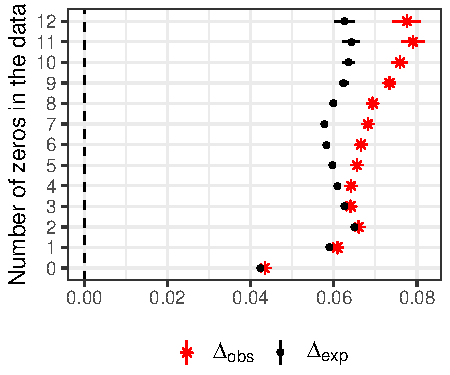
\includegraphics[scale=0.85]{margins/splithalf_n250000_figa1}
	\end{subfigure}%
	\begin{subfigure}{.45\textwidth}
		\centering	
		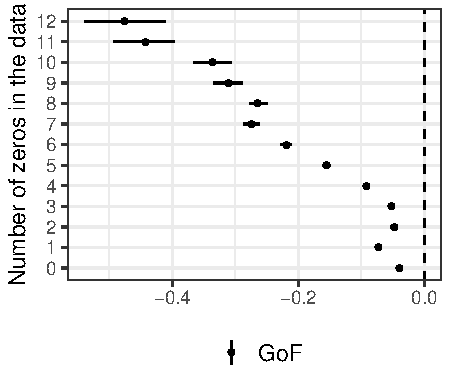
\includegraphics[scale=0.85]{margins/splithalf_n250000_figa2}
	\end{subfigure}
	\caption{Correlation between the appearance of zeros in the data, and goodness-of-fit. Best model was selected according to AIC.}
	\label{fig:splithalf_n250000_figa1}
\end{figure}

\begin{figure}[!t]
	\begin{subfigure}{1\textwidth}
		\centering
		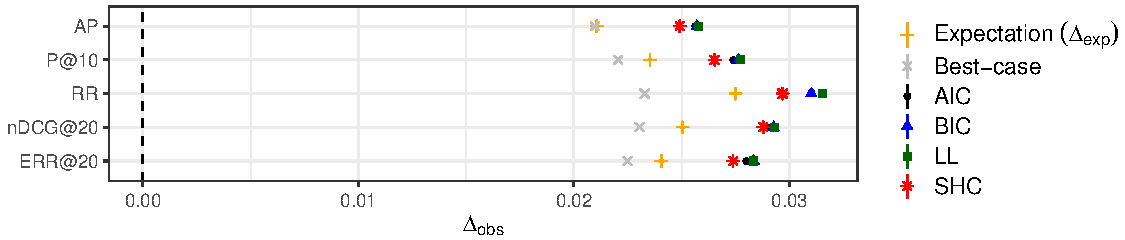
\includegraphics[scale=0.85]{margins/splithalf_n250000_fig4}
		\caption{Overall results.}
		\label{fig:margins-splithalf-plot-4}
	\end{subfigure} \newline
	\begin{subfigure}{1\textwidth}
		\centering
		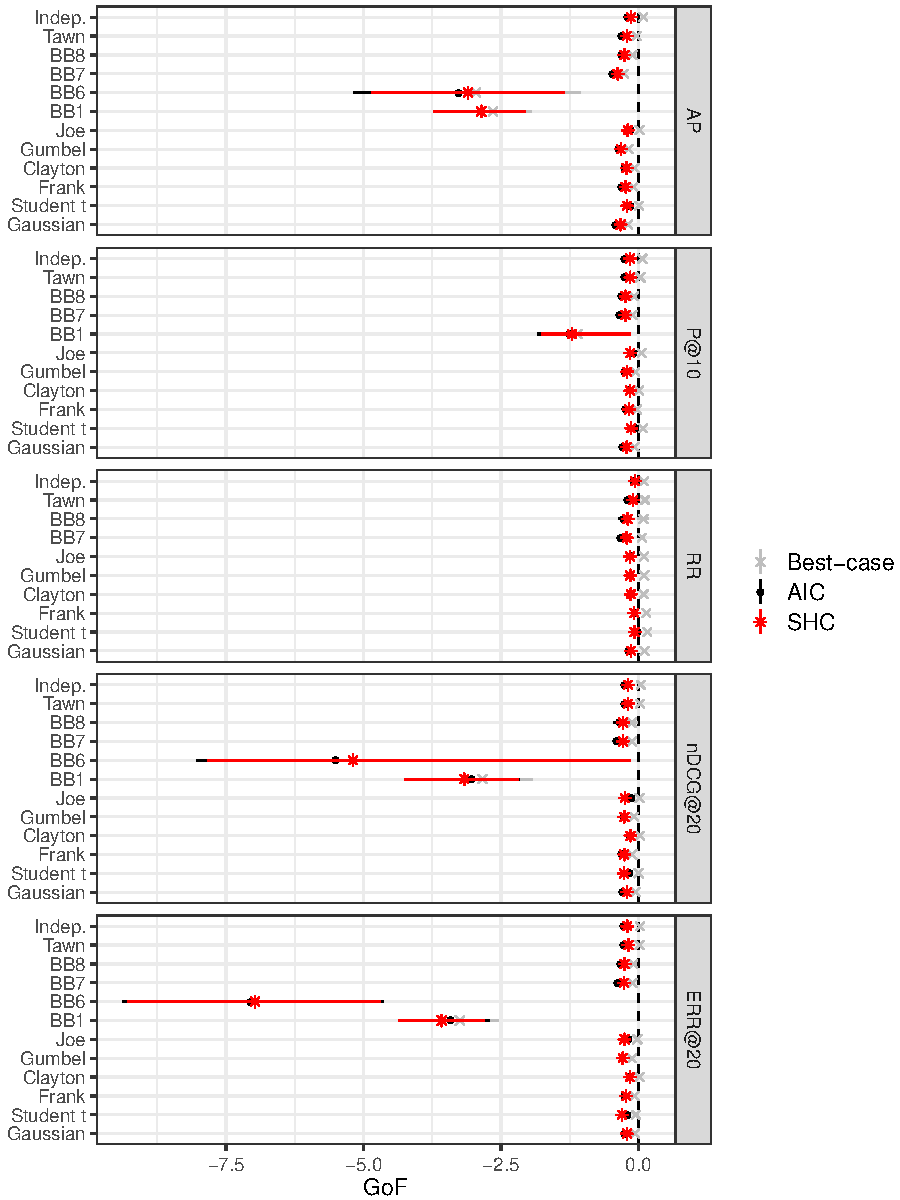
\includegraphics[scale=0.85]{margins/splithalf_n250000_fig5}
		\caption{Breakdown of the results based on the alternative candidate model that would have been selected.}
		\label{fig:margins-splithalf-plot-5}
	\end{subfigure}
	\caption{For those cases where AIC ranked Beta KS \nth{1}, how would the \nth{2} or \nth{3} best models perform, if they had been selected?}
	\label{fig:margins-splithalf-plot-4,5}
\end{figure}

\begin{figure}[!t]
	\centering	
	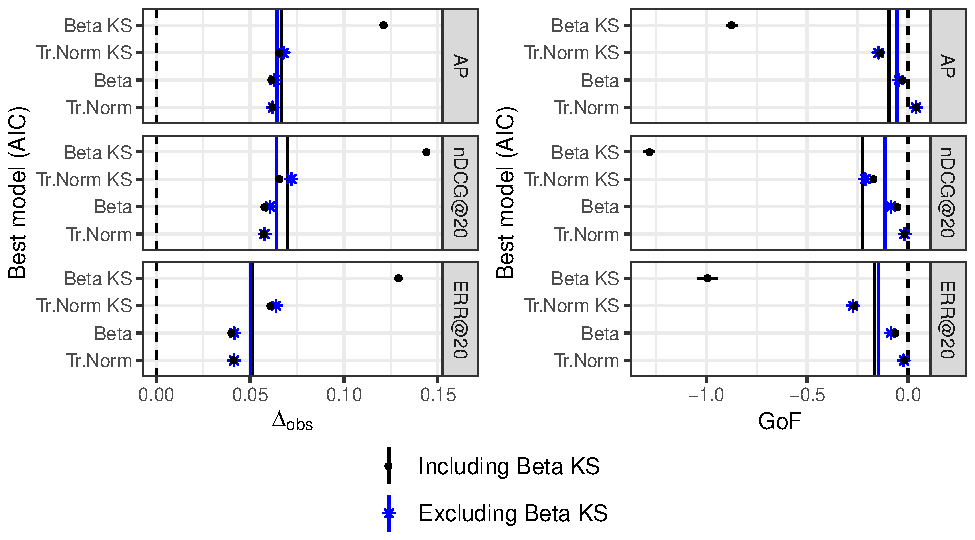
\includegraphics[scale=0.85]{margins/splithalf_n250000_fig6c}
	\caption{How would the goodness-of-fit of the marginal models be affected, if we had removed the Beta KS distribution from the list of candidates? The vertical lines indicate overall means across measures.}
	\label{fig:margins-splithalf-plot-6}
\end{figure}

\clearpage 


\subsection{Comparing Model Selection Criteria}

So far we have solely focused on AIC as a model selection criterion, as done in \cite{Urbano2019}. This criterion provides a balance between simple and underfitted models, and complex and overfitted models. However, we found that this selection is not always satisfactory, as we identified a specific set of corner cases where AIC tends to make poor choices. Moreover, our findings regarding the quality of the margins do suggest that there could be room for improvement. In the top plot of Figure \ref{fig:margins-splithalf-plot-8}, we see that our overall $\Delta_{\text{obs}}$ measurements, even with the improvement that we achieved by removing Beta KS from the list of candidates, is higher than the expectation across all continuous metrics. More specifically, looking at the bottom plot, we see that the $\Delta_{\text{obs}}$ is about 10\% higher than the expectation, for the case of continuous metrics. Ideally we would have hoped for values slightly closer to zero, which means that the quality can be improved. Moreover, we demonstrate that \textit{if} the models had been selected optimally (shown as 'best-case'), the GoF would have been much better. Of course, selecting models in an optimal manner is virtually impossible, however, it does show some potential for improving the quality of the margins, without adding new distributions families to the current list of candidate models. It is therefore meaningful to explore alternative ways of selecting the models that we already have. 

\begin{figure}[t]
	\begin{subfigure}{1\textwidth}
		\centering
		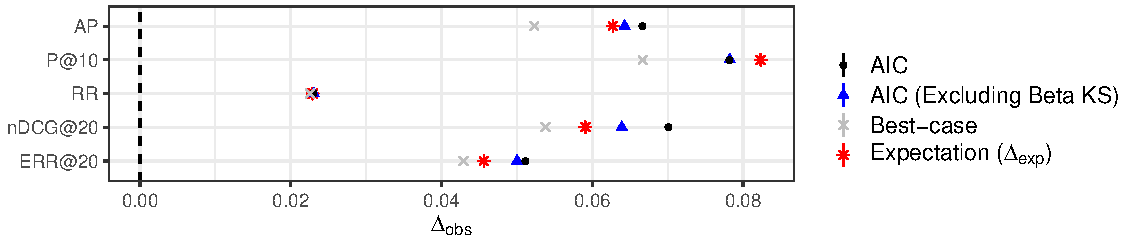
\includegraphics[scale=0.85]{margins/splithalf_n250000_fig8}
	\end{subfigure} \newline
	\begin{subfigure}{1\textwidth}
%		\centering
		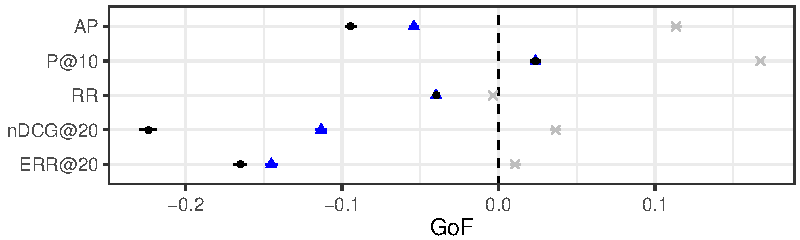
\includegraphics[scale=0.85]{margins/splithalf_n250000_fig8b}
	\end{subfigure}
	\caption{The overall mean $\Delta_{\text{obs}}$ and GoF that is measured, when the models are selected by \textit{i)} AIC, \textit{ii)} AIC with the removal of Beta KS from the list of candidates, and \textit{iii)} optimally, by choosing the model with the lowest $\Delta_{\text{obs}}$ in each random split.}
\label{fig:margins-splithalf-plot-8}
\end{figure}

In this context, we developed and experimented with a new model selection criterion, which we propose in this thesis. Our proposed criterion, is inspired by the split-half approach, and we denote it as SHC (Split-Half Criterion). In Figure \ref{fig:SHC_diagram}, we illustrate how this criterion works, through an example. Starting with a set of scores (in this case 25 AP scores), we repeatedly split the data in half, $n$ times. If the original data contain 25 scores, then the first half will contain 12 scores, and the second half will contain the remaining 13. For each split, we fit all possible models on the first half of the data, and then, using the empirical distribution of the second half of the data as ground-truth, we compute a $\Delta_{\text{obs}}$ for each model. For example, in the first trial split, we observed a delta of $0.21$ for Beta KS, and $0.18$ for the Truncated Normal distribution respectively. In total, we repeat this process $n$ times. In the end, to compute the SHC of a model that is fitted on the entire set of 25 scores, say Beta KS, we simply average the $\Delta_{\text{obs}}$ values that we measured for Beta KS across all $n$ splits. For example, for the case of Beta KS, we compute its value like so: $SHC_{\text{Beta  KS}}=\left(0.21+...+0.05\right)/n$. Essentially, the purpose of each split, is to give us an estimate of what the performance might look like for a given marginal distribution family, on the \textit{entire} set of 25 scores. The more splits we perform, the better our estimate should be. In the end, the best model according to SHC, is the one with the lowest SHC value.

%\begin{equation}\label{eq:shc}
%	SHC_{\text{family f}} = \sum_{i=1}^{n}\frac{\Delta_\text{obs}^{\text{family f, split i}}}{n}  
%\end{equation}

\begin{figure}[t]
	\centering	
	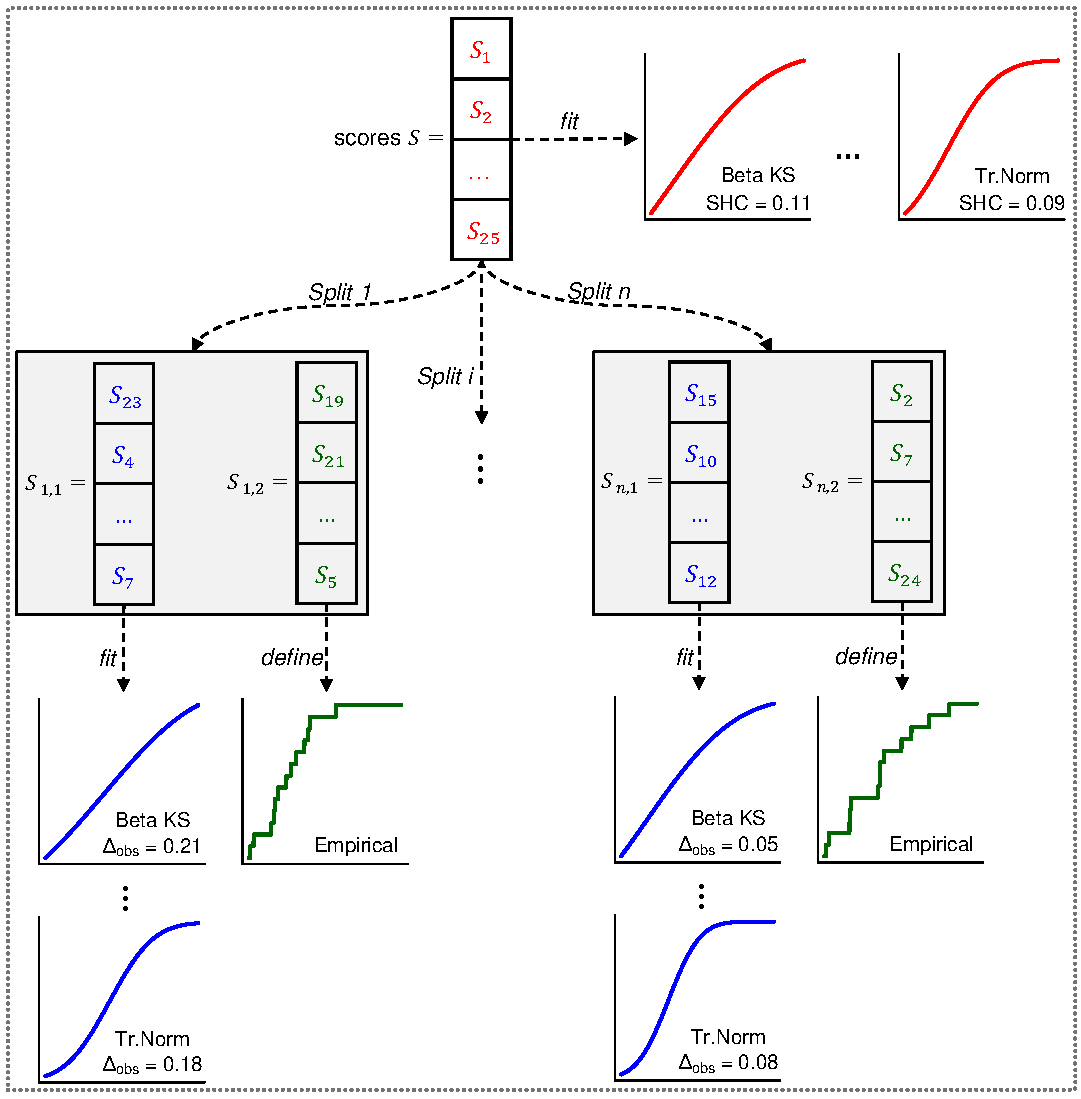
\includegraphics[width=0.9\linewidth]{../diagrams/diag4_SHC}
	\caption{Diagrammatic representation of how the Split-Half Criterion (SHC) is computed.}
	\label{fig:SHC_diagram}
\end{figure}

\begin{figure}[!t]
	\begin{subfigure}{1\textwidth}
		\centering
		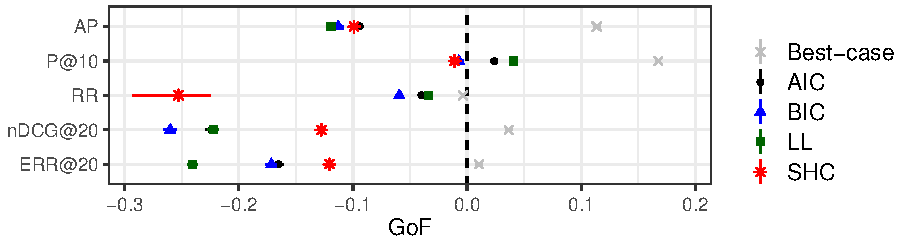
\includegraphics[scale=0.84]{margins/splithalf_n250000_fig9a_gof}
		\caption{Including Beta KS.}
		\label{fig:margins-splithalf-plot-9a}
	\end{subfigure} \newline
	\begin{subfigure}{1\textwidth}
		\centering
		\hspace*{-.17\textwidth}
		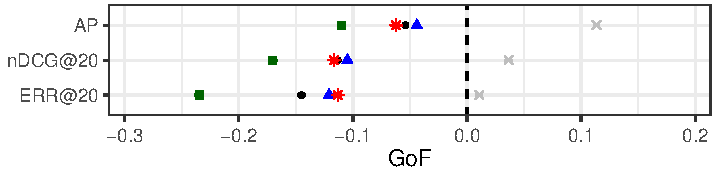
\includegraphics[scale=0.84]{margins/splithalf_n250000_fig9b_gof}
		\caption{Excluding Beta KS.}
		\label{fig:margins-splithalf-plot-9b}
	\end{subfigure}
	\caption{Comparison of the model selection criteria, in terms of overall mean GoF that is measured.}
	\label{fig:margins-splithalf-plot-9}
\end{figure}

In Figure \ref{fig:margins-splithalf-plot-9}, we compare the performance of well established model selection criteria, namely LL, AIC and BIC (Equations \ref{eq:LL}-\ref{eq:BIC}), in terms of the overall mean GoF that we measured with them. On top of these criteria, we also include our newly proposed criterion, SHC, and set its parameter for the number of splits at $n=10$. This comparison was performed on the same \num{250000} random splits that we previously created. The results for $\Delta_{\text{obs}}$, are completely analogous, however we plot GoF values to make the visual interpretation of the results easier, due to the fact that changes in absolute $\Delta_{\text{obs}}$ can be difficult to distinguish. In the top plot, Beta KS was included in the list of candidates, whereas in the bottom plot it was excluded; meaning, that in any event where some selection criteria ranked Beta KS \nth{1}, we simply selected the \nth{2} best model. The exclusion of Beta KS improves the overall mean GoF, regardless of the criterion that was used. In the top plot, we see that for the case of discrete metrics (P@10 and RR) all criteria perform well, with only one exception for SHC in the case of RR. For the case of continuous metrics (AP, nDCG@20 and ERR@20), SHC performs the best overall. In the bottom plot, we see that when Beta KS is excluded (which is something that affects all continuous metrics), all criteria perform very similarly, with the exception of LL. In summary, these results suggests that, the overall goodness-of-fit is maximized by excluding Beta KS from the list of candidates, in combination with using AIC or BIC. Furthermore, we can conclude that, since we did not observe a significant improvement with any of these criteria, to further improve the goodness-of-fit of the margins, beyond the exclusion of Beta KS, would likely require to enrich to the list of candidates with additional models.
 
 %In Figure \ref{fig:determine-n-for-shc} we show the overall mean goodness-of-fit that is achieved, when the models are selected based on SHC, for various $n$ parameters. 
 
 %\begin{figure}[t]
 %	\centering	
 %	\includegraphics[width=0.75\linewidth]{}
 %	\caption{Diagrammatic representation of the approach used for computing $\Delta_\text{obs}^{25}$ and $\Delta_\text{obs}^{50}$.}
 %	\label{fig:determine-n-for-shc}
 %\end{figure}

\subsection{Extrapolating Results to Larger Topic Set Sizes}

Even though the split-half approach has the advantage that it remains true to the data, it suffers from the fact that the data are being halved. For example, in our case, the main goal is to measure the goodness-of-fit of marginal models that are fitted on the \textit{entire} set of (50) topic-scores, however, in a split-half approach, half of the data are held-out to provide an estimate of the ground truth. This means that we actually measure the goodness-of-fit of models that are fitted on only \textit{half} (25) of those topic-scores. For this reason, we want to know if we underestimate or overestimate the goodness-of-fit, and by how much. In other words, we want to extrapolate our findings to a larger topic set size. To accomplish this, we require data collections that contain more topics. One of those collections is the one from the Terabyte TREC Track of 2006 (Table \ref{tab:dataset-descriptive-stats-terabyte}), which contains the scores of various systems on 149 topics. The large number of topic-scores that is present in this collection, allows us to repeatedly split the data in three sets of scores, as shown in Figure \ref{fig:diag5}. The first two sets are obtained by randomly splitting the entire set of scores in two, so that one split contains 50 scores ($S_{50}$), and the other split contains the remaining 99 scores ($S_{99}$). The third set, $S_{25}$, is obtained by randomly sampling 25 scores from $S_{50}$. By doing so, we can fit one model ($F_{25}^*$) on $S_{25}$ and another model ($F_{50}^*$) on $S_{50}$. Then, using the empirical distribution of $S_{99}$ as an estimate of the ground truth, we can compute $\Delta_\text{obs}^{25}$ and $\Delta_\text{obs}^{50}$, respectively, for the two models.

\begin{table}[t]
	\centering
	\begin{tabular}{l c c c l}
		\toprule
		TREC Track & Years & \#Systems & \#Topics & Effectiveness Measures \\
		\midrule
		Terabyte & 2006 & 61 & 149 & \{AP, RR, P@10\} \\
		\bottomrule
	\end{tabular}
	\caption{Some descriptive statistics about the Terabyte collection.}
	\label{tab:dataset-descriptive-stats-terabyte}
\end{table} 

\begin{figure}[t]
	\centering	
	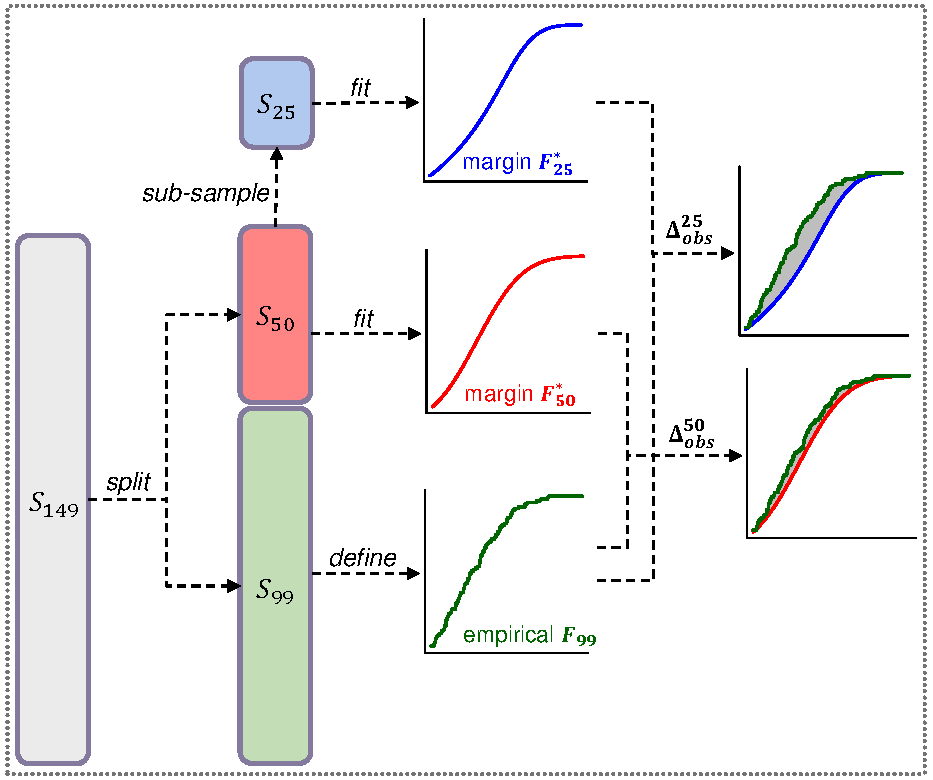
\includegraphics[width=0.75\linewidth]{../diagrams/diag5}
	\caption{Diagrammatic representation of the approach used for computing $\Delta_\text{obs}^{25}$ and $\Delta_\text{obs}^{50}$.}
	\label{fig:diag5}
\end{figure}

In Figure \ref{fig:margins-extrapolate-plot-1} we report the $\Delta_\text{obs}^{25}$ and $\Delta_\text{obs}^{50}$ values that we measured, in \num{150000} trials. All models were selected according to AIC. Overall, our results show that when models are fitted on 50 topics, as opposed to 25, they measure a $\Delta_\text{obs}$ that is slightly lower. This suggests that our split-half approach actually tends to underestimate the goodness-of-fit of the marginal models, by a small amount. This occurrence seems to be consistent across all distribution families, however, we notice an outlier, that once again involves the Beta KS distribution. In those particular cases where this distribution is chosen (in the case of 25 topics), the performance is underestimated by a large amount. Interestingly, in this particular dataset, Beta KS is actually never selected in the case of 50 topics; although, this is not the case with other datasets, as we saw earlier in Figure \ref{fig:margins-splithalf-plot-3}. Table \ref{tab:margins-extrapolate-table-1} shows that, on average, for the case of AP and P@10, $\Delta_\text{obs}^{50}$ is 7.6\% and 2.8\% smaller than $\Delta_\text{obs}^{25}$, respectively. For the case of RR, it is 63.8\% larger; however, in absolute terms, this difference is quite negligible, since both $\Delta_\text{obs}^{50}$ and $\Delta_\text{obs}^{25}$ tend to be very low. In summary, these results show that our split-half approach tends to slightly underestimate the goodness-of-fit of the marginal models. 

\begin{figure}[!t]
	\centering	
	\begin{subfigure}[t]{.33\textwidth}
		\centering
		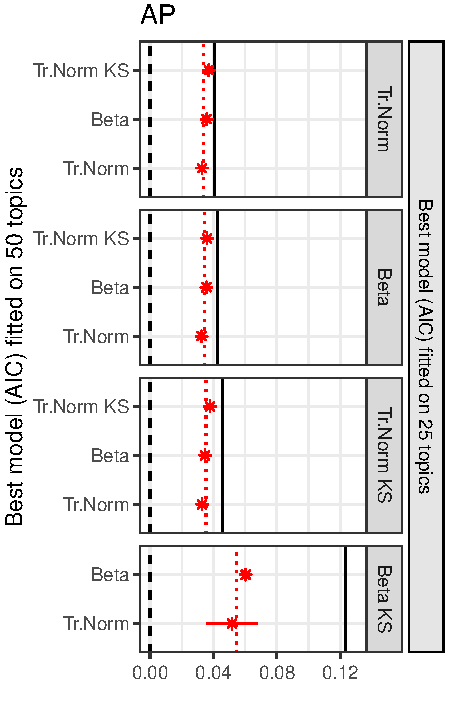
\includegraphics[width=.99\linewidth,valign=t]{margins/extrapolate_n150000_fig1_ap}
	\end{subfigure}%
	\begin{subfigure}[t]{.33\textwidth}
		\centering
		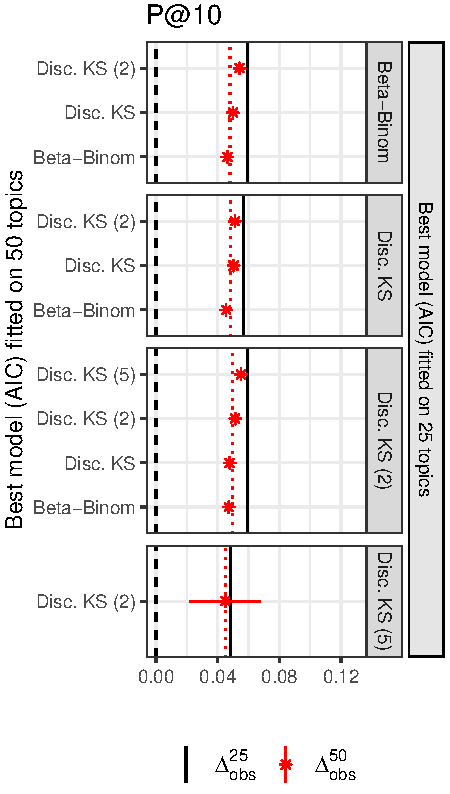
\includegraphics[width=.99\linewidth,valign=t]{margins/extrapolate_n150000_fig1_p10}
	\end{subfigure}
	\begin{subfigure}[t]{.33\textwidth}
		\centering
		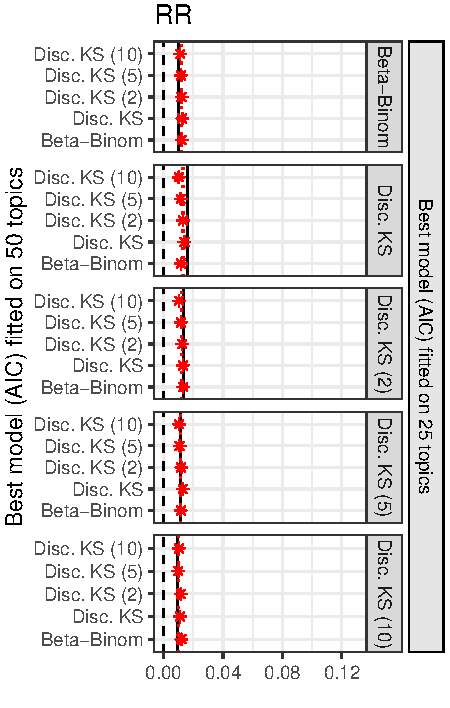
\includegraphics[width=.99\linewidth,valign=t]{margins/extrapolate_n150000_fig1_rr}
	\end{subfigure}
	\caption{How different would our $\Delta_\text{obs}$ measurements be, if the marginal models had been fitted on 50 topics, as opposed to 25?}
	\label{fig:margins-extrapolate-plot-1}
\end{figure}

\clearpage

\begin{table}[t]
	\centering
	\begin{tabular}{c c}
		% middle column is all italic
		\toprule
		& $\overline{\left(\frac{\Delta_\text{obs}^{50} - \Delta_\text{obs}^{25}}{\Delta_\text{obs}^{25}}\right)}$ \\ \midrule
		AP    & -0.076       \\
		P@10  & -0.028       \\
		RR    &  0.638       \\ \bottomrule
	\end{tabular}
	\caption{How different is $\Delta_\text{obs}^{50}$ compared to $\Delta_\text{obs}^{25}$?}
	\label{tab:margins-extrapolate-table-1}
\end{table}

\subsection{Summary of Results}

Summarizing our results, we found that the marginal models fit the data moderately well, when they are selected by AIC, with the exception of the Beta Kernel Smoothing distribution. The goodness-of-fit of the models that are fitted on discrete metrics (P@10 and RR) is noticeably better than those fitted on continuous metrics (AP, nDCG@20 and ERR@20). Also, the models are selected similarly in 25 topics, compared to 50 topics, which gives us some confidence regarding the accuracy of our goodness-of-fit estimates. Moreover, due to the fact that all candidate families get selected, and no particular family gets chosen with a significantly higher frequency than the rest; this implies that IR data are indeed complex.

The Beta Kernel Smoothing distribution is an obvious outlier, that on average, measures a $\Delta_{\text{obs}}$ twice that of our expectation. We explored this further and found that part of the explanation behind this is the high appearance of zero scores in the data. Although, there are other particularities about those corner case, which we did not manage to detect. It appears that Beta KS models tend to be too simple and underfitted to capture these types of data, yet they are still selected by AIC. 

In an attempt to correct this outlier, we found that the exclusion of Beta KS from the list of candidates, notably improves the overall GoF, from -0.22 to -0.11, for the case of nDCG@20, which is the case where Beta KS is selected the most. Interestingly, we discovered that even if the models were selected optimally, none of the candidate families would have performed up to standard, in those particular cases where AIC selected Beta KS. This implies that in order to further improve the quality of the margins in those specific cases, beyond the exclusion of Beta KS, more candidate models would have to be considered. One of such models, could be a mixture model that models the zero scores separately from non-zeros. We leave this for future work.

In an attempt to refine the quality of the margins, instead of focusing on expanding the list of candidate models with additional ones, we experimented with alternative ways of selecting them, including AIC, BIC and LL. We also proposed a new selection criterion that is inspired by the split-half approach, which we denote as SHC (Split-Half Criterion). We found that for the case of continuous metrics (especially nDCG@20), SHC selects models considerable better than the other criteria, although, for the case of discrete metrics (especially RR), it performs considerably worse. However, we found that the best approach for maximizing the overall goodness-of-fit of the margins, is to simply exclude Beta KS from the list of candidates, and select models based on either AIC or BIC. This approach works more consistently across the different effectiveness metrics.

In a separate, smaller scale experiment, we determined that our estimates regarding $\Delta_{\text{obs}}$ are underestimated by 7.6\%, 2.8\% for AP and P@10 respectively. For the case of RR we overestimate by 63.8\%, however, in absolute terms, it is a negligible value.









